\chapter{Ocean Surface Modeling}
To capture the physical behavior of electromagnetic waves reflecting off the surface of the ocean, we need to model the surface altitude variations correctly. For this, we first need to understand the power spectra of ocean waves and their dependencies. Next, we can generate random realizations of sea surfaces by discretizing the power spectrum and taking the inverse Fourier transform of a Hermitian sequence of spectrally appropriate coefficients.

\section {Waves in the Ocean}
Ocean waves are primarily driven by wind and start when turbulence creates capillary or surface waves with small wavelengths (on the order of a few centimeters). As the wind continues to blow, it increases both the amplitude and the wavelength of the waves until they start to interact. These interactions continue to increase the wavelength and phase speed of the waves until they are traveling faster than the wind, at which point the sea is fully developed. As a sea develops, the energy will transfer from higher frequencies to lower frequencies by the processes just described.

Before discussing the statistical properties of ocean waves, it is useful to review some standard nomenclature. Fetch is the length over which the wind can be considered constant, and a longer fetch generally means higher waves. Significant wave height is the mean wave height of the highest third of the waves. Significant wave height is represented in the literature as $H_{1/3}$ and is equal to 4 times the standard deviation of the wave height, $H_{1/3} = 4\sigma_h$.

The phase speed of wves due to gravity in deep water is $v_p=\sqrt{g/k}$, which allows us to write the dispersion relation $\omega = \sqrt{gk}$. This dispersion relation is import for changing variables in the power spectra, for instance converting $S(\omega)$ to $S(k)$. We can use the fact that the amount of energy contained per unit interval should be constant so that $S(k)dk = S(\omega)d\omega = S(f)df$. To convert a power spectrum in terms of $\omega$ to one in terms of $k$, we would use the expression in Equation \ref{os_eq:0aa}.

\begin{equation}
  \label{os_eq:0aa}
  S(k) = S(\omega = \sqrt{qk})\frac{d\omega}{dk}
  \end{equation}

\section{Ocean Wave Power Spectra}  \label{os_sec:power_spectra}
Many methods have been proposed to statistically describe the behavior of ocean waves. These range from the simplest sea state representation with a very coarse binning of wind speed and sea height variations to the mathematically complex Elfouhaily variance power spectrum that unifies the more recent work.

\subsection {Sea State}
The modern concept of sea state is a combination of the Beaufort wind scale and the Douglas sea scale. The Beaufort scale was developed in the early 1800s by sir Francis Beaufort and the Douglas scale was developed in the 1920s by H.P Douglass, both of the Royal Navy \cite{uk_met_fact_sheet6}. Table \ref{os_tab:0} shows the World Meterological Organization (WMO) sea state vs. wind speed, with wave height referring to the mean difference between successive peaks and throughs (twice the amplitude).

\begin{table}[H]
\begin{center}
  \begin{tabular} {|c | c | c| c|}
    \hline
  \bf{Sea State} & \bf{Descriptio}n & \bf{Wave Height (m)} & \bf{Wind Speed (m/s)}\\ \hline
  0 & Calm (glassy) & 0 & $<$ 0.3 \\ \hline
  1 & Calm (rippled) & 0 - 0.1 & 0.3 - 1.5 \\ \hline
  2 & Smooth (wavelets) & 0.1 - 0.5 & 1.6 - 3.3 \\ \hline
  3 & Slight & 0.5 - 1.25 & 3.4 - 5.5 \\ \hline
  4 & Moderate & 1.25 - 2.5 & 5.5 - 10.7 \\ \hline
  5 & Rough & 2.5 - 5 & 10.8 - 13.8 \\ \hline
  6 & Very Rough & 4 -6 & 13.9 - 17.1\\ \hline
  7 & High & 6 - 9 & 17.2 - 24.4\\ \hline
  8 & Very High & 9 - 14 & 24.5 - 32.6\\ \hline
  9 & Phenomenal & $\geq$ 14 & $\geq$ 32.7\\ \hline
\end{tabular}
  \renewcommand{\baselinestretch}{1} \small\normalsize
  \begin{quote}
    \caption[WMO Sea State vs. Wind Speed]{WMO Sea State vs. Wind Seed\label{os_tab:0}}
  \end{quote}
\end{center}
\end{table}
\renewcommand{\baselinestretch}{2} \small\normalsize

\subsection{Pierson-Moskowitz Spectrum}
In 1964, the Pierson-Moskowitz (PM) spectrum defined in Equation \ref{os_eq:1} was developed to describe the power spectrum of the variance of wave height and relate it to the measured wind speed 19 meters above the sea surface ($U_{19}$) and the coefficient of gravity ($g=9.81 m/s^2$) \cite{michel_sea_spectra}. 
 \begin{equation}
S(k) = \frac{0.0081}{k^3}e^{-0.74\left(\frac{g}{k}\right)^2U_{19}^{-4}}
\label{os_eq:1}
\end{equation}
 \renewcommand{\baselinestretch}{2} \small\normalsize
 The PM power spectrum ($S$) is shown in the left hand side of Figure \ref{os_fig:1} and the associated curvature spectrum ($k^3S$) is shown in the right hand side of Figure \ref{os_fig:1}. These figures were generated for wind speeds from 3 m/s to 21 m/s in increments of 2 m/s.
 
 \begin{figure}[H]
  \begin{center}
\includegraphics[width=6in]{../media/PM_variance_curvature_spectrum.png}
  \end{center}
  \renewcommand{\baselinestretch}{1} \small\normalsize
  \begin{quote}
    \caption[Pierson-Moskowitz Variance and Curvature Spectra]{Pierson-Moskowitz Variance and Curvature Spectra\label{os_fig:1}}
  \end{quote}
\end{figure}
 \renewcommand{\baselinestretch}{2} \small\normalsize
 
The PM spectrum assumes deep water, infinite fetch and no swells and has repeatedly been shown to be accurate for gravity waves in fully developed seas, but fails to capture spectral peaks due to high winds over short fetches. This means that the low frequency component of the power spectrum is valid in almost all cases but the high frequency component is not, as can be seen by the flat slope of both $S$ and $k^3S$ in Figure \ref{os_fig:1}.

\subsection{Bretschneider Spectrum}
To overcome the limitations of a spectrum that required fully developed seas, several multi-parameter spectra were developed. In 1978, the 12th International Towing Tank Conference recommended the two-parameter Bretschneider spectrum given in Equation \ref{os_eq:1a} where the modal frequency $\omega_m$ is given by $\omega_m = 0.4\sqrt{g/H_{1/3}}$.
\begin{equation}
  \begin{gathered}
  \label{os_eq:1a}
  S(k) = \frac{1.25 \omega_m^4}{8k^3g^2}e^{-1.25\frac{\omega_m^4}{g^2k^2}} 
  \end{gathered}
\end{equation}
\renewcommand{\baselinestretch}{2} \small\normalsize

\subsection{JONSWAP Spectrum}
Join North Sea Wave Project in the 1970s modified the Pierson-Moskowitz spectrum by adding a peak enhancement factor as shown in Equation \ref{os_eq:1b} \cite{michel_sea_spectra}.
\begin{equation}
  \label{os_eq:1b}
  S(k) = S_{PM}(k)\nu^{\frac{k-k_0}{2\sigma^2k_0}} 
  \end{equation}
The enhancement factor $\nu$ was empirically derived for many locations in the North Sea.

\subsection{Elfouhaily Spectrum}
Many additional spectra have been developed and in 1997, Elfouhaily et. al unified several of these to provide a modern spectrum that is broken into low and high frequency regions, $B_l$ and $B_h$, \cite{elfouhaily}.
\begin{equation}
  \label{os_eq:2}
  S(k) = k^{-3}\left[B_l + B_h \right]
\end{equation}
\renewcommand{\baselinestretch}{2} \small\normalsize
The Elfouhaily spectrum is dependent on the wind speed at 10 m altitude ($U_{10}$) and the inverse age parameter ($\Omega$). The inverse age parameter indicates how developed the sea is; fully developed for $\Omega = 0.84$, mature for $\Omega = 1.0$, and young for $\Omega > 2.0$. 

The low frequency region, $B_l$, is given by Equation \ref{os_eq:3} and the parameters are defined in Table \ref{os_tab:1}.
\begin{equation}
  \label{os_eq:3}
 B_l = \frac{1}{2} \alpha_p \frac{c_p}{c} F_p
\end{equation}
\renewcommand{\baselinestretch}{2} \small\normalsize
\begin{subequations}
   Low frequency spectrum dependencies:
\begin{align*}
  F_p &= L_{PM}J_pe^{-\Omega\left[\sqrt{10}\left(\sqrt{k/_{k_p}} - 1 \right) \right]^{-1}} &  k_p &= g\left(\frac{\Omega}{U_{10}}\right)^2 & c_p &= \frac{U_{10}}{\Omega} \\
   L_{PM} &=e^{-\frac{5}{4}\left(\frac{k}{k_p} \right)^2} &  J_p &= \gamma^\Gamma  & \alpha_p &= 0.006\Omega^{0.55} 
\end{align*}
\end{subequations}
\renewcommand{\baselinestretch}{2} \small\normalsize
\begin{table}[H]
\begin{center}
  \begin{tabular} {|c | c |}
    \hline
  \bf{Parameter} & \bf{Description} \\ \hline
  $F_p$ & Long wave side effect function \\ \hline
  $k_p$ &  Wave number of the spectral peak \\ \hline
  $c_p$ &  Phase speed at the spectral peak \\ \hline
  $L_{PM}$ & PM shape spectrum \\ \hline
  $J_p$ & JONSWAP peak enhancement function \\ \hline
   $\alpha_p$ & Generalized Phillips-Kitaigorodskii long wave equilibrium range parameter\\ \hline
\end{tabular}
  \renewcommand{\baselinestretch}{1} \small\normalsize
  \begin{quote}
    \caption[Elfouhaily Low Frequency Spectrum Parameters]{Elfouhaily Low Frequency Spectrum Parameters\label{os_tab:1}}
  \end{quote}
\end{center}
\end{table}
\renewcommand{\baselinestretch}{2} \small\normalsize
The high frequency region, $B_h$, is given by Equation \ref{os_eq:4} and the parameters are defined in Table \ref{os_tab:2}.
\begin{equation}
  \label{os_eq:4}
 B_h = \frac{1}{2} \alpha_m \frac{c_m}{c} F_m
\end{equation}
\renewcommand{\baselinestretch}{2} \small\normalsize
\begin{subequations}
   Low frequency spectrum dependencies:
\begin{align*}
  F_m &= L_{PM}J_pe^{-\frac{1}{4}\left[k/_{k_m} - 1 \right]^2 } & k_m & = 370 \text{ rad/m} &  c_m &=\sqrt{\frac{2g}{k_m}} \\
  u^* &= \sqrt{0.00144}U_{10}  & \alpha_m &= \alpha_o\frac{u^*}{c_m}  \\
  L_{PM} &=e^{-\frac{5}{4}\left(\frac{k}{k_p} \right)^2}  &  J_p &= \gamma^\Gamma
\end{align*}
\end{subequations}
\renewcommand{\baselinestretch}{2} \small\normalsize
\begin{table}[H]
\begin{center}
  \begin{tabular} {|c | c |}
    \hline
  \bf{Parameter} & \bf{Description} \\ \hline
  $F_m$ & Short wave side effect function \\ \hline
  $k_m$ &  Wave number at the secondary peak of the curvature spectrum \\ \hline
  $c_m$ &  Minimum phase speed at $k_m$ \\ \hline
  $\alpha_m$ & Generalized Phillips-Kitaigorodskii short wave equilibrium range parameter \\ \hline
  $L_{PM}$ & PM shape spectrum \\ \hline
  $J_p$ & JONSWAP peak enhancement function \\ \hline
\end{tabular}
  \renewcommand{\baselinestretch}{1} \small\normalsize
  \begin{quote}
    \caption[Elfouhaily High Frequency Spectrum Parameters]{Elfouhaily High Frequency Spectrum Parameters\label{os_tab:2}}
  \end{quote}
\end{center}
\end{table}
\renewcommand{\baselinestretch}{2} \small\normalsize
The variables $L_{PM}$ and $J_p$ are found in both $B_l$ and $B_h$ and are given by Equations \ref{os_eq:5}.
\begin{equation}
\begin{gathered}
  \label{os_eq:5}
    \gamma = \begin{cases}
    1.7,& \text{if } 0.84 < \Omega < 1\\
    1.7 + 6\log{\Omega}, & \text{if } 1 < \Omega < 5
  \end{cases} \\
  \Gamma = \exp{\left[- \frac{\left(\sqrt{\frac{k}{kp} - 1} \right)}{2\sigma^2} \right]} \\
  \sigma = 0.08\left[1 + 4\Omega^{-3} \right] \\
\end{gathered}
\end{equation}
\renewcommand{\baselinestretch}{2} \small\normalsize
To compare the results, the Elfouhaily and PM variance spectra are shown in the left hand side of Figure \ref{os_fig:2} for wind speeds of 5 m/s and 10 m/s. The inverse age parameter was set to 0.84 to match and the wind speed at 19 m was approximated from $U_{19} \approx 1.026 U_{10}$. The Elfouhaily spectra are shown by the dashed lines and indicate a deviation from the PM spectra at large wave numbers. The corresponding curvature spectra are shown in the right hand side of Figure \ref{os_fig:2}. The secondary peak in the Elfouhaily curvature spectrum is shown at 370 rad/m.
\begin{figure}[H]
  \begin{center}
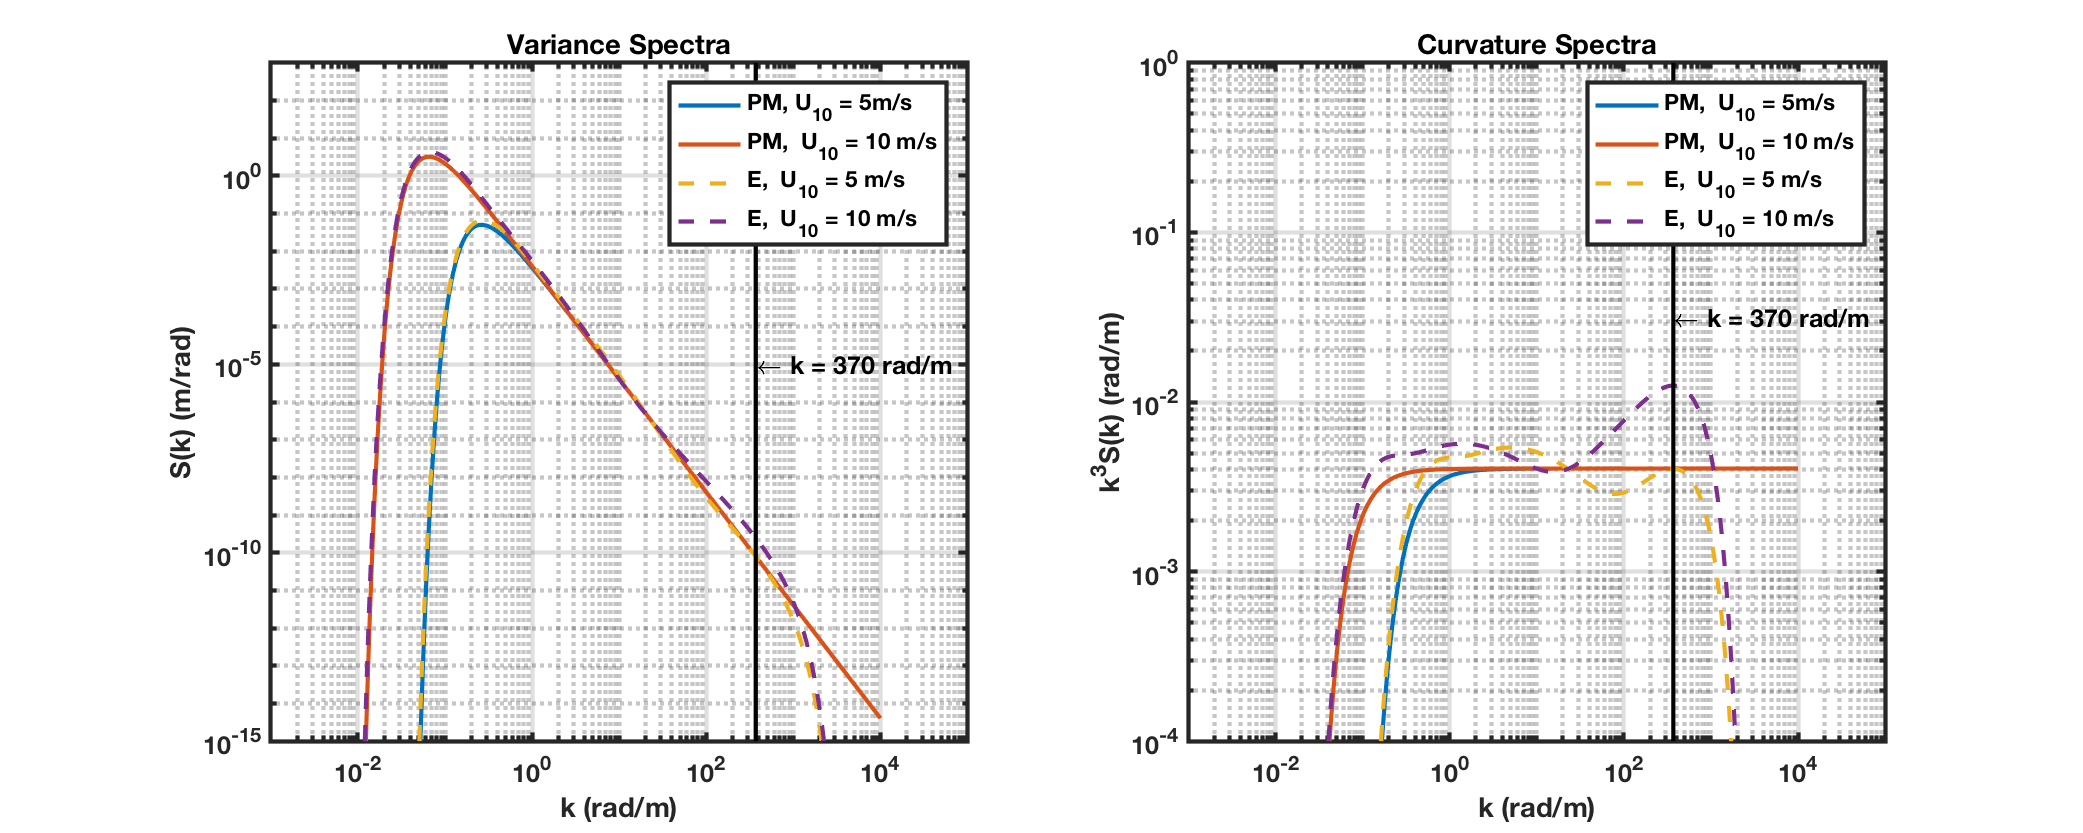
\includegraphics[width=6in]{../media/elf_vs_PM_variance_curvature_spectrum.png}
  \end{center}
  \renewcommand{\baselinestretch}{1} \small\normalsize
  \begin{quote}
    \caption[Elfouhaily vs. Pierson Moskowitz Variance and Curvature Spectra]{Elfouhaily vs. Pierson Moskowitz Variance and Curvature Spectra\label{os_fig:2}}
  \end{quote}
\end{figure}
\renewcommand{\baselinestretch}{2} \small\normalsize
To look at the dependence on wind speed, the Elfohaily variance spectrum is shown in the left hand side of Figure \ref{os_fig:3} and the associated curvature spectrum is shown in the right hand side of Figure \ref{os_fig:3}. These figures were generated for wind speeds from 3 m/s to 21 m/s in increments of 2 m/s, matching Figure 8 in \cite{elfouhaily}.
\begin{figure}[H]
  \begin{center}
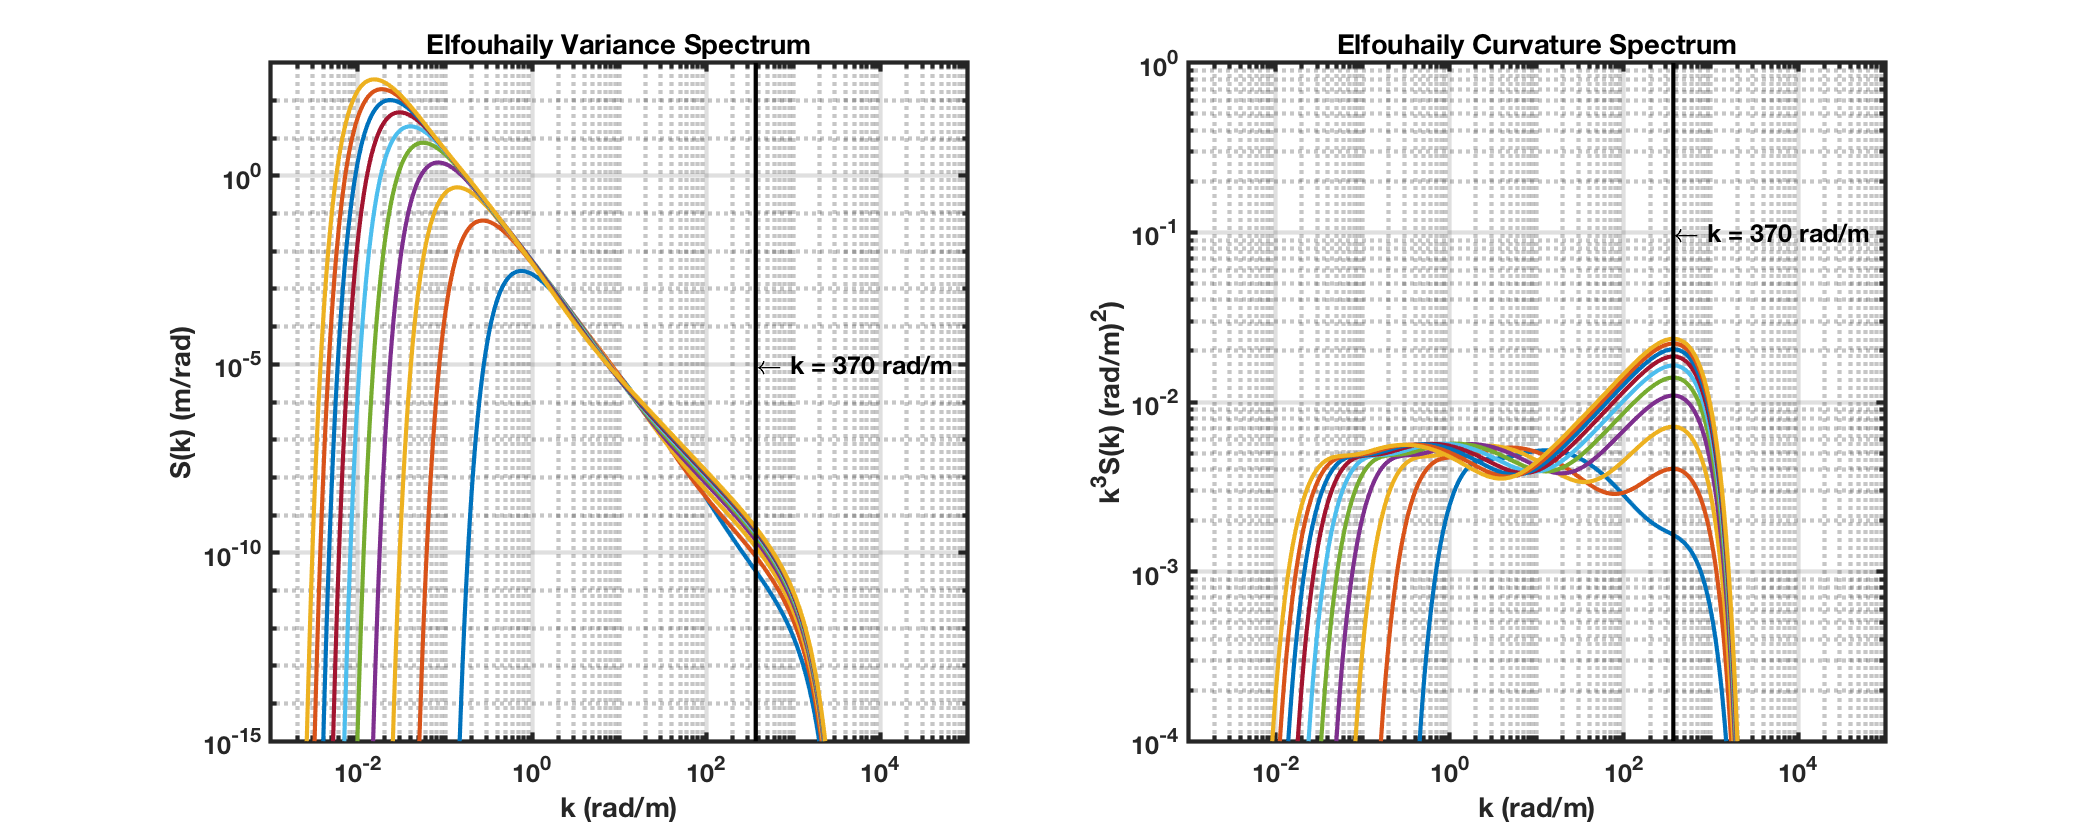
\includegraphics[width=6in]{../media/elf_variance_curvature_spectrum.png}
  \end{center}
  \renewcommand{\baselinestretch}{1} \small\normalsize
  \begin{quote}
    \caption[Elfouhaily Variance and Curvature Spectra]{Elfouhaily Variance and Curvature Spectra\label{os_fig:3}}
  \end{quote}
\end{figure}
\renewcommand{\baselinestretch}{2} \small\normalsize

\subsection{Directional Spreading Functions}
All the variance power spectra that have been discussed are uni-directional, meaning they only apply downrange in the direction of the wind. For two-dimensional surfaces, we need to include angular extent.

\section{Generation of Sea Surface Realizations}
Realizations of sea surfaces rely on adequate sampling to cover the spectral range of interest and then generating an appropriate set of Fourier coefficients.

\subsection{Sampling Constraints}
In order to generate a random sea surface height realization,  the first thing we need to establish is the number of points to use, $N$, and the spatial domain length to cover, $L$. These parameters define the geometry and sampling of the problem.The spatial domain sampling is given as $\Delta x = \frac{L}{N}$ and the frequency domain sampling is  given as $\Delta k = \frac{2\pi}{L}$.

The highest wave number that can be sampled given these values is $k_{max} = \frac{N}{2}\Delta k = \frac{N\pi}{L} = \frac{\pi}{\Delta x}$ rad/m, which corresponds to a minimum wavelength of $\lambda_{min} = 2\Delta x = \frac{2L}{N} = \frac{4\pi}{\Delta k N}$ m.

\subsection{Power Spectrum Discretization}
We next follow the procedure outlined in \cite{percival_spectra},  where we work in the frequency domain and start with a set of Gaussian distributed random variables, $W_j$. We need to scale these random numbers by the square root of the Elfouhaily variance spectrum, arrange them so the sequence is Hermitian, and then take the inverse Fourier transform. For a sequence of $N$ variables, and a two-sided continuous power spectrum, $S(k)$, we can generate the frequency domain random variables, $V(k)$ as shown in Equation \ref{os_eq:6}.
\begin{equation}
  \label{os_eq:6}   
  V_j = \begin{cases}
    \sqrt{S_0}W_0, & j = 0 \\
    \sqrt{\frac{1}{2}S_j}\left(W_{2j-1} + iW_{2j} \right), & 1 \leq j <\frac{N}{2} \\
    \sqrt{S_{N/_2}}W_{N-1}, & j = \frac{N}{2} \\
    V_{N-j}^*, &  \frac{N}{2} < j \leq N-1 
  \end{cases} 
\end{equation}
Since we have a one-sided, discrete power spectrum, there are some additional scaling factors that need to be added to Equation \ref{os_eq:6} for conservation of energy. To convert to a discrete power spectrum, we use the fact that the amount of energy contained per unit interval will be a constant, so that $S(f)df = S(k)dk = S(\omega) d\omega$. To normalize the spectrum to the specified wave number sampling interval, we simply need to multiply by $\Delta k$. Next, since we have a one-sided spectrum rather than a two-sided one, we have half the energy and need to divide the power spectrum by 2. With these factors included, we can define the discrete spectrum as $Sd(k) = \frac{S(k)\Delta k}{2}$.

In order to understand the remaining scale factors and evaluate the 2nd moment, we can rewrite Equation \ref{os_eq:6} into a more clear form as shown in Equation \ref{os_eq:7}, letting $u(k) = W_{2-j}$ and $v(k) = W_{2j}$.
\begin{equation}
  \begin{gathered}
  \label{os_eq:7}
  V(+k) = \sqrt{\frac{1}{2}}\left[u(k) + iv(k) \right]\sqrt{S_d(k)} \\
  V(-k) = \sqrt{\frac{1}{2}}\left[u(-k) - iv(-k) \right]\sqrt{S_d(-k)}
  \end{gathered}
\end{equation}
The 2nd moment of either of these functions individually is equal to $S_d(k)$, but the 2nd moment of the combined function is $2S_d(k)$. This means we need to multiply the sequence $V(k)$ by an additional scale factor of $\sqrt{\frac{1}{2}}$ to conserve the total energy. We could also arrive at this result by realizing that in Equation \ref{os_eq:7}, we are starting with a sequence of length $N/2$ and extending it to cover a length of $N$, effectively doubling the energy contained. The scaling factor corrections are shown in Equation \ref{os_eq:8}.
\begin{equation}
  \label{os_eq:8}   
  V_j = \begin{cases}
    \sqrt{\frac{1}{2}S_0\Delta k}W_0, & j = 0 \\
    \sqrt{\frac{1}{2}S_j\Delta k}\frac{1}{2}\left(W_{2j-1} + iW_{2j} \right), & 1 \leq j < \frac{N}{2} \\
    \sqrt{\frac{1}{2}S_{N/_2}\Delta k}W_{N-1}, & j = \frac{N}{2} \\
    V_{N-j}^*, &  \frac{N}{2} < j \leq N-1 
  \end{cases} 
\end{equation}
Now that we have the random Fourier coefficients, we can generate the sea surface through the inverse Fourier transform. Because the sequence is Hermitian, the sea surface will be purely real.
\begin{equation}
  \label{os_eq:9}
  h(x) = \mathcal{F}^{-1}\left\{V(k) \right\}
  \end{equation}

\subsection{Example Realizations}
Figure \ref{os_fig:7} shows one realization of a sea surface with $U_{10}$ = 20 m/s, $N$ = $2^{20}$, and $L$ = 10 km. For these parameters, $\Delta x$ = 9.5 mm, $\Delta k$ = 0.628 mrad/m, $k_{max} = 32.9\times 10^4$ rad/m, and $\lambda_{min} = 19$ mm.
\begin{figure}[H]
  \begin{center}
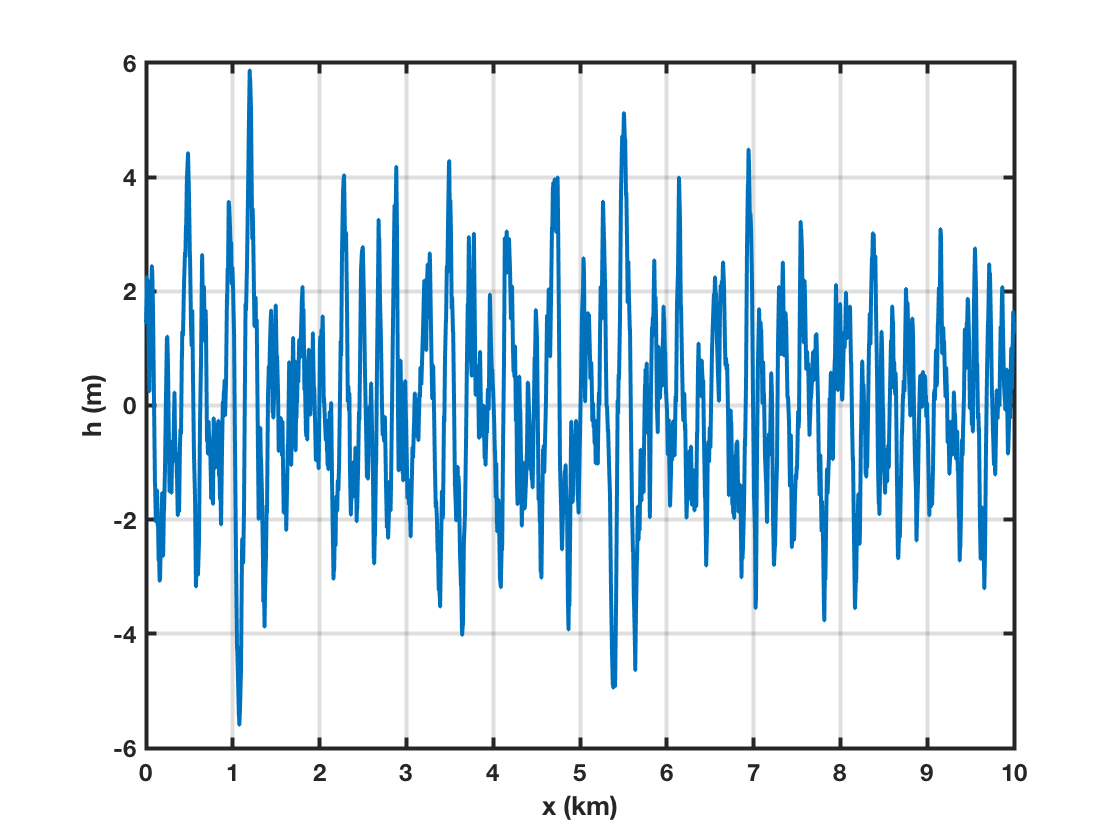
\includegraphics[width=5in]{../media/realized_sea_surface_20m_per_s.png}
  \end{center}
  \renewcommand{\baselinestretch}{1} \small\normalsize
  \begin{quote}
    \caption[Sea Surface Realization with $U_{10}$ = 20 m/s]{Sea Surface Realization with $U_{10}$ = 20 m/s\label{os_fig:7}}
  \end{quote}
\end{figure}
\renewcommand{\baselinestretch}{2} \small\normalsize
Figure \ref{os_fig:8} shows the original variance spectrum and the locations of the sampling points in wave number space.
\begin{figure}[H]
  \begin{center}
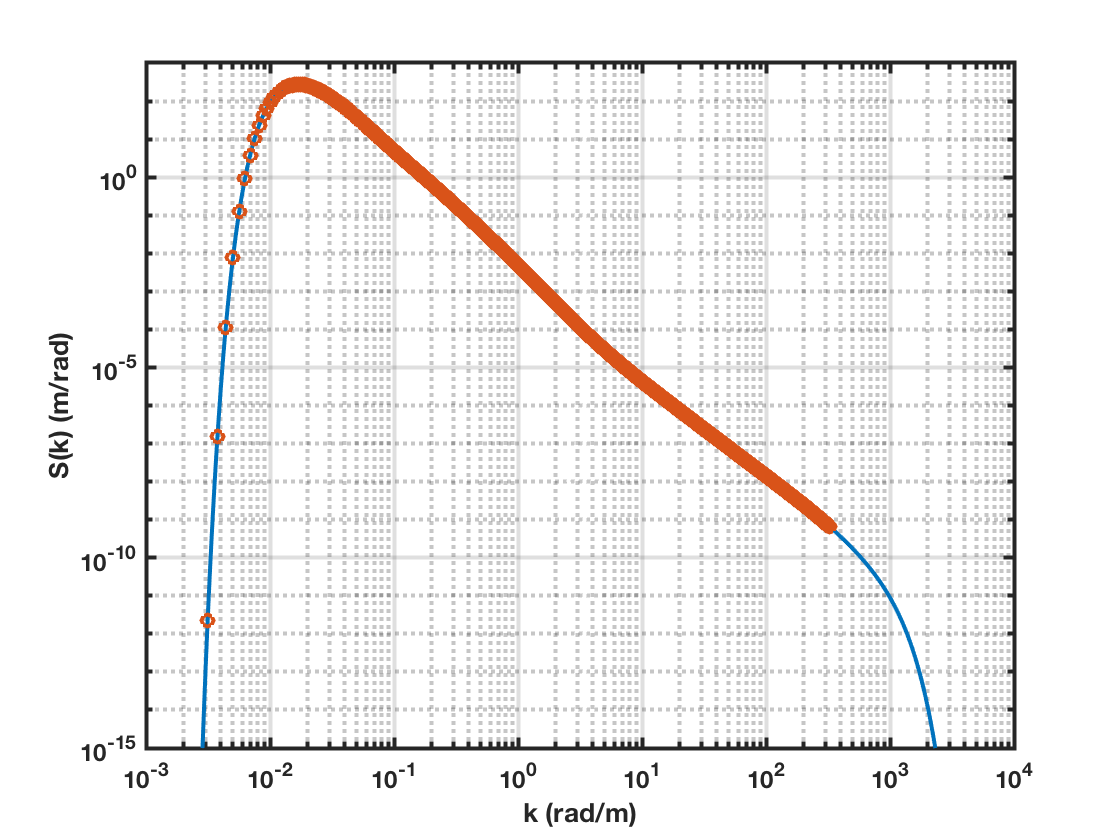
\includegraphics[width=5in]{../media/sampled_spectra_points.png}
  \end{center}
  \renewcommand{\baselinestretch}{1} \small\normalsize
  \begin{quote}
    \caption[Elfouhaily Variance Spectrum Showing Sampled Points]{Elfouhaily Variance Spectrum Showing Sampled Points\label{os_fig:8}}
  \end{quote}
\end{figure}
\renewcommand{\baselinestretch}{2} \small\normalsize
Figure \ref{os_fig:9} shows the original variance spectrum compared to the recovered spectrum that was estimated from the sea surface realization.
\begin{figure}[H]
  \begin{center}
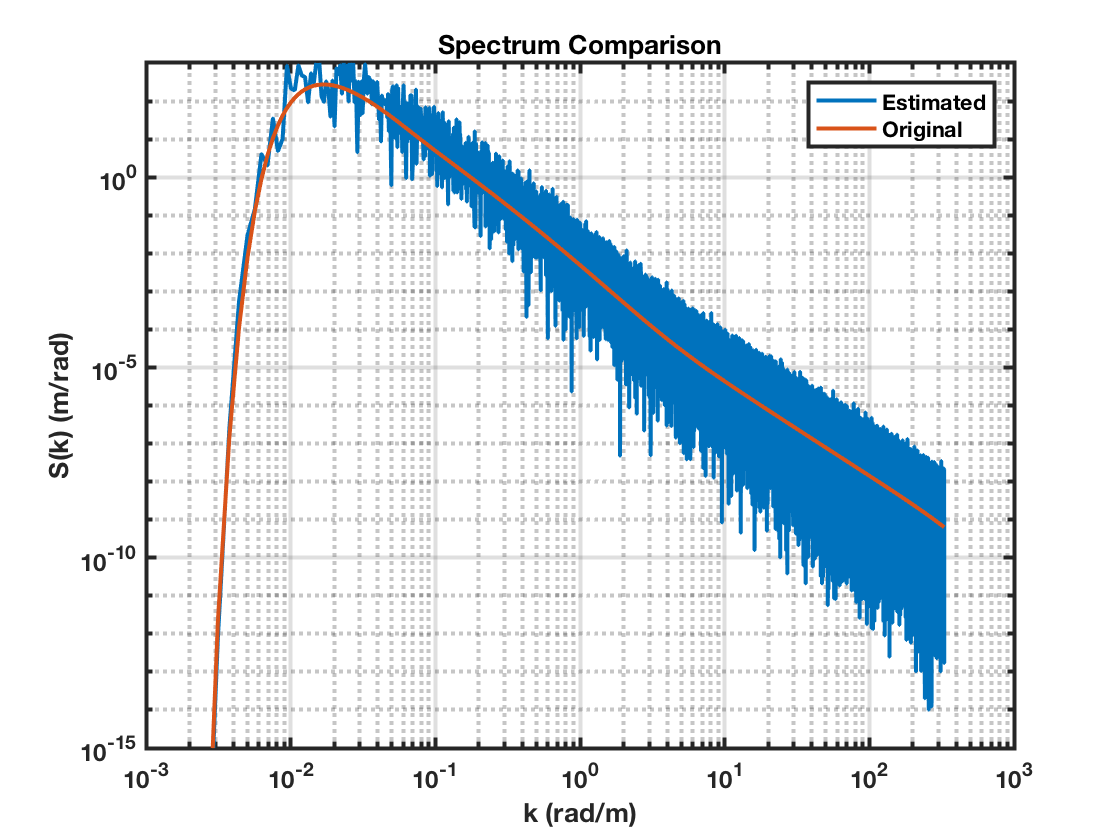
\includegraphics[width=5in]{../media/recreated_test_spectrum.png}
  \end{center}
  \renewcommand{\baselinestretch}{1} \small\normalsize
  \begin{quote}
    \caption[Comparison of Original and Recovered Spectra]{Comparison of Original and Recovered Spectra\label{os_fig:9}}
  \end{quote}
\end{figure}
\renewcommand{\baselinestretch}{2} \small\normalsize
